\documentclass[a4paper,11pt]{article}


% Please do not change the packages and commands listed here. You can of course add your favourite packages and commands.

%%% Pakete %%% 

\usepackage{graphicx}
\usepackage{amsmath}
\usepackage[utf8]{inputenc}
\usepackage{enumerate}
\usepackage{amsthm}
\usepackage{amssymb}
\usepackage{paralist}
\usepackage{dsfont}
\usepackage{booktabs}
\usepackage{tabularx}
\usepackage{hyperref}
\usepackage{mathtools}
\usepackage{verbatim}
\usepackage{ dsfont }
\usepackage{ xcolor }
\usepackage{environ}
\usepackage{lipsum}
\usepackage{multirow}



%%% Additional Commands %%%

%% These commands might mak it easier for you to write formal statements.

\newcommand{\N}{\ensuremath{\mathds{N}}} % natural numbers
\newcommand{\Z}{\ensuremath{\mathds{Z}}} % integers
\newcommand{\Q}{\ensuremath{\mathds{Q}}} % rational numbers
\newcommand{\R}{\ensuremath{\mathds{R}}} % real numbers

\newcommand{\states}{\ensuremath{\mathcal{S}}} % state space
\newcommand{\actions}{\ensuremath{\mathcal{A}}} % action space
\newcommand{\policy}{\ensuremath{\pi}} % a policy
\newcommand{\stateval}{\ensuremath{v}} % state value function
\newcommand{\actionval}{\ensuremath{q}} % action value function
\newcommand{\optsval}{\ensuremath{v_*}} % state value function
\newcommand{\optaval}{\ensuremath{q_*}} % action value function

\newtheorem{lemma}{Lemma}
\newtheorem{example}{Example}
\theoremstyle{definition}
\newtheorem{prob}{Exercise}
\newtheorem{pcode}{Pseudocode}




% -----------------------------
\begin{document}

%%% TITLE PAGE %%%
%   - Please only modify your name(s) and do not change anything else! %

\begin{titlepage}
\pagestyle{empty}
  \begin{minipage}[t]{0.6\textwidth}
    \begin{flushleft}
      \bf 
      Reinforcement Learning and Decision Making Under Uncertainty\\
    \end{flushleft}
  \end{minipage}\hfill
  \begin{minipage}[t]{0.3\textwidth}
    \begin{flushright}
      \bf Spring 2022\\
      Jakub Tłuczek, Lukas Zoller
    \end{flushright}
  \end{minipage}

	\medskip

  \begin{center}
    {\Large\bf Project Report}
    
  {\bf Submission Deadline: 03 June 2022, 14:00}
    \Large
    \vspace{2cm}
    
    %%% ENTER THE NAMES OF GROUP MEMBERS HERE %%%
    %
    {Group:}\\
    {JAKUB TŁUCZEK}\\
    {LUKAS ZOLLER}
    
    \vspace{2cm}
    \begin{tabular}[b]{|l|r|}
    \hline
    Introduction, Related Work, Preliminaries &\qquad\qquad/\;\;5\\\hline
    Structure, Notation, Formal correctness &\qquad\qquad/\;\;5\\\hline
    Main Content and Explanations &\qquad\qquad/30\\\hline 
    Discussion \& Conclusion&\qquad\qquad/10\\\hline
    $\Sigma$&\qquad\qquad/50\\\hline
    \end{tabular}
  \end{center}
\end{titlepage}
%%% END TITLE PAGE %%%


%%% Useful hints %%%


%%%%%%%%%%%%%%%%%%%%%%%%%%%%%%%%%%%%%%%%%%%%%%%%%%%%%%%%%%%%%%%%%%%%
%%%%%%%%%%%%%%%%%%%%%%%%%%%%%%%%%%%%%%%%%%%%%%%%%%%%%%%%%%%%%%%%%%%%
%%%%%%%%%%%%%%%%%%%%%%%%%%%%%%%%%%%%%%%%%%%%%%%%%%%%%%%%%%%%%%%%%%%%
% From here on we give a sample structure of a report. You can modify this structure as you wish.
%%%%%%%%%%%%%%%%%%%%%%%%%%%%%%%%%%%%%%%%%%%%%%%%%%%%%%%%%%%%%%%%%%%%
%%%%%%%%%%%%%%%%%%%%%%%%%%%%%%%%%%%%%%%%%%%%%%%%%%%%%%%%%%%%%%%%%%%%
%%%%%%%%%%%%%%%%%%%%%%%%%%%%%%%%%%%%%%%%%%%%%%%%%%%%%%%%%%%%%%%%%%%%

\newpage
\pagestyle{plain}
\pagenumbering{arabic}


\section{Introduction}
This project report summarizes the practical project of the course "Reinforcement Learning and Decision Making Under Uncertainty" at the University of Neuchâtel in the spring semester of 2022, prepared by Jakub Tłuczek and Lukas Zoller.

The aim of the project was to implement a Reinforcement Learning algorithm on a frozen lake like environment\footnote{https://github.com/openai/gym/blob/master/gym/envs/toy\_text/frozen\_lake.py} with additional complications. Our environment models a sea with enemies our agent (the pirate) has to avoid and merchant ships the agent has to catch. Upon finding itself on the same field as enemy or merchant, agent obtains negative or positive reward respectively. Each step made by agent also cost it a small negative reward. Agent has limited field of view, in our work set to 5x5 grid.

Placement of vessels on the sea is random, therefore it might be the case that some initial states are easier to solve than others. Ultimate goal is to train an agent in a robust way, to take this randomness, as well as movement of vessels on the sea, into account.

\section{Preliminaries}
The environment has been programmed from scratch. We didn't deviate from the original plan, which was:


\begin{quote}
Our environment represents a quadratic sea map where a pirate (the agent) wants to rob and destroy merchant ships. Each merchant ship will return a positive reward. If the agent robs all merchant ships, the game will be over. It will also be over after fixed amount of moves. There are also enemy ships moving on the map which the agent has to avoid. If the agent is on the same field as an enemy ship the game will also be over with a negative reward for the agent.\footnote{Cited from the project proposal}
\end{quote}

\clearpage

\paragraph{Map}
The following shows a representation of our map with the following encoding: -1 = outside map, 0 = empty sea, 1 = pirate (our agent), 2 = merchant ship, 3 = pirate ship.

\begin{verbatim}
 -1 -1 -1 -1 -1 -1 -1 -1 -1
 -1 -1 -1 -1 -1 -1 -1 -1 -1
 -1 -1  1  0  0  0  3 -1 -1
 -1 -1  0  0  0  2  0 -1 -1
 -1 -1  0  0  0  0  2 -1 -1
 -1 -1  0  0  3  0  0 -1 -1
 -1 -1  0  0  0  0  0 -1 -1
 -1 -1 -1 -1 -1 -1 -1 -1 -1
 -1 -1 -1 -1 -1 -1 -1 -1 -1
\end{verbatim}

\paragraph{State}
\label{sec:state}
The agent \say{perceives} the environment which lies inside a certain distance around him. If the agent has a visibility distance of 2, with the above example map he see the following:
 \begin{verbatim}
 -1 -1 -1 -1 -1 
 -1 -1 -1 -1 -1 
 -1 -1  1  0  0 
 -1 -1  0  0  0  
 -1 -1  0  0  0 
\end{verbatim}
The agent will receive this state as a flattened vector.

\paragraph{Flexible environment parameterization} 
Our environment can be changed quite easily with the setting of the following parameters:
\begin{itemize}
	\item size of the environment (side length of the square) 
	\item number of enemies (fixed or random)
	\item number of merchants (fixed or random)
	\item if the enemies and merchants shall move or if they stay at the same spot over the whole episode.
	\item algorithm parameters 
\end{itemize}
These parameters can be easily changed with the config file and allow us to run experiments more easily. 

\section{Main Content}
While looking for the main method, an article \cite{crabe_2020} based on \cite{schaul_2016} brought an inspiration to use Deep Q-Networks with Priority Experience Replay (later referred to as DQN with PER) in our project. 

\subsection{Main method - DQN with PER}

Two features appealed to us in particular - first is the usage of neural networks, which addresses the robustness fears, second is the novel way how are the experiences sampled from the buffer - namely based on its sampling probability and weight:

\begin{align*}
    P(i) = \frac{p_i^{\alpha}}{\Sigma_k p_k^{\alpha}} \;\;\;\;\;
    w_i = (\frac{1}{N} \frac{1}{P(i)})^{\beta}
\end{align*}

Experiences are sampled according to probability $P(i)$, which in turn depends on priorities $p_i$, which are obtained according to loss function after forward pass of the neural network. Weights are calculated based on said probabilities, and are introduced in order to eliminate bias in backward pass, as data was not sampled uniformly in the first place (hence introducing the bias). Additionally there are two parameters, $\alpha$ and $\beta$ which battle the overfitting at the end of training - alpha decays as training goes on, with beta growing at the same time. 

Full algorithm, as presented in \cite{schaul_2016}:

\begin{figure}[h]
    \centering
    \includegraphics[width=13cm]{algorithm.png}
    \caption{Deep Q-Learning with prioritized experience replay}
    \label{fig:my_label}
\end{figure}

At each step, algorithm first observes the transition that happened and stores it in buffer with maximal priority. In some intervals, specified as parameters, experiences are first sampled from the buffer as minibatches. Afterwards, sampling weights are computed beforehand, for them to be ready for backward pass. Loss is obtained after forward pass, and subsequently priority is updated to reflect it. Finally, network weights (not to confuse with sampling weights) are updated after minibatch calculations finish. Afterwards, action is selected based on current policy and loop repeats. 

\subsection{Baseline methods}

While looking for baseline methods, first idea was to compare Deep Q-Learning with its traditional counterpart, which uses Q-table to optimize its policy. Upon realizing that state space and action space would result in enormous Q-table ($4*5^{24}$), we decided to look for another method to compare this with. Briefly we considered using Fourier Basis approximation \cite{ziemke_2020}, however we ultimately didn't find it suitable for this project.\\
Our choice was another off-policy algorithm, namely Soft Actor Critic \cite{haarnoja_2018}. Resulting state space would still be large, therfore we decided to choose implementation based on neural networks as well. OpenAI, who are the authors of popular benchmark framework for reinforcement learning Gym \url{gymlibrary.ml}, have also produced framework for deep reinforcement learning called SpinningUp \url{spinningup.openai.com}. Unfortunately, project seems to be abandoned since 2020, therefore in order to make it work with our environment, we had to modify extensively the source code for SAC, available at \footnote{https://github.com/openai/spinningup/tree/master/spinup/algos/pytorch/sac}. \\
Regrettably, in case of our environment this method didn't converge, therefore we switched our focus to ablation tests - that is, how does the main method perform when:

\begin{itemize}
    \item sampling weights are calculated (full PER algorithm)
    \item sampling weights are not calculated (all sampling weights are set to 1)
    \item experiences are sampled uniformly from the buffer
\end{itemize}

\subsection{Experiments}
\label{sec:experiments}
In order to test all scenarios, experiments have been conducted by running each scenario 5 times, scoring the returns in queue with fixed size N and each $\frac{N}{10}$ steps plotting the average return during past N episodes. We have chosen N to be 100.\\
Results of training were then plotted, with each point representing mean return of the last N epochs. Lines represent the mean values at each point, while shaded areas in the same color denote standard deviation at that point.\\

\begin{figure}[h]
    \centering
    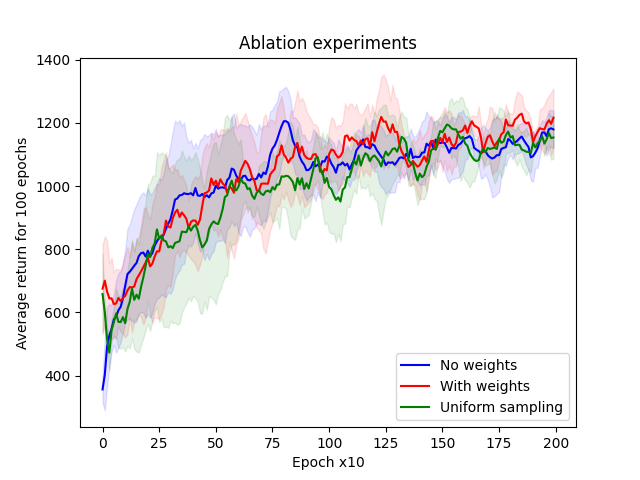
\includegraphics[width=12cm]{experiment.png}
    \label{fig:my_label}
\end{figure}
\\
During training phase each scenario seems to perform just as well, although deviations in first 250-500 epochs seems to be fairly large.\\
Finally, models in each scenario (which were saved to a state dictionary beforehand), were loaded and ran 1000 times each to get an average return. Later, to check whether there is a statistical evidence that there is a difference in means of each scenario, Student's t-test was performed for every pair of scenarios.

\begin{center}
    \begin{tabular}{|c|c|c|c|c|c|c|c|c|}
        \hline
        \multirow{2}{*}{Scenario} & \multirow{2}{*}{\mu} & \multirow{2}{*}{\sigma} & \multicolumn{2}{c|}{Weights} &
        \multicolumn{2}{c|}{No weights} &
        \multicolumn{2}{c|}{Uniform}\\
        \cline{4-9}
        & & & t & p & t & p & t & p\\
        \hline
        Weights & 1020.46 & 698.15 & - & - & 0.23 & 0.82 & 0.51 & 0.61\\
        \hline
        No weights & 1027.73 & 712.14 & 0.23 & 0.82 & - & - & -0.73 & 0.47\\
        \hline
        Uniform & 1004.25 & 716.03 & 0.51 & 0.61 & -0.73 & 0.47 & - & -\\
        \hline
    \end{tabular}
\end{center}

In each case it fails to reject null hypothesis, that true means are equal. Therefore, there is not enough statistical evidence to show, that any of this method is superior to another.

\subsection{Lunar Lander experiments}

In \cite{crabe_2020} author used the environment Lunar Lander \footnote{https://github.com/openai/gym/blob/master/gym/envs/box2d/lunar\_lander.py}. We also checked, how does the algorithm perform in this specific environment.\\
Since we didn't have computational power and time to perform experiments as we did in the case of our environment, we ran each scenario once, and then compared both training progresses and evaluations, done 1000 times each on saved state dictionaries of models produced in each scenario.\\


\begin{figure}[h]
    \centering
    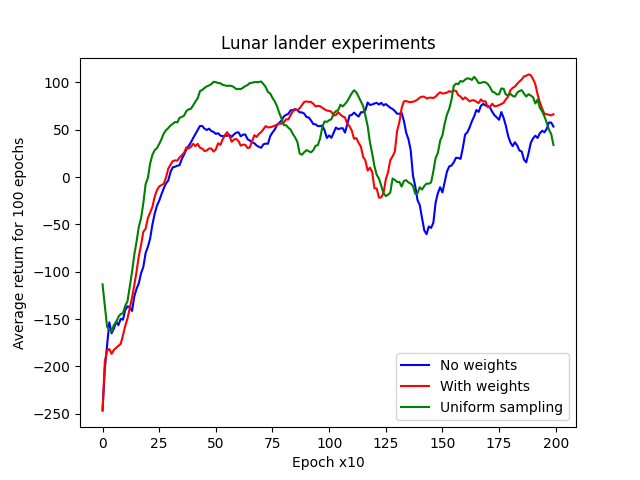
\includegraphics[width=12cm]{experiment_ll.png}
    \label{fig:my_label}
\end{figure}
\\

We observed that during training, in each scenario there were periods with much worse score than before. These drops were sudden, and promptly came back to the level one thought they might be converging on. In further work, it would be interesting to explain this phenomenon.\\

We have also evaluated scores of training agent in similar fashion as in \hyperref[sec:experiments]{Experiments}.\\

\begin{center}
    \begin{tabular}{|c|c|c|c|c|c|c|c|c|}
        \hline
        \multirow{2}{*}{Scenario} & \multirow{2}{*}{\mu} & \multirow{2}{*}{\sigma} & \multicolumn{2}{c|}{Weights} &
        \multicolumn{2}{c|}{No weights} &
        \multicolumn{2}{c|}{Uniform}\\
        \cline{4-9}
        & & & t & p & t & p & t & p\\
        \hline
        Weights & 0.67 & 147.43 & - & - & 8.53 & 5e-17 & 5.23 & 2e-7\\
        \hline
        No weights & 71.97 & 223.66 & 8.53 & 5e-17 & - & - & -11.73 & 7e-30\\
        \hline
        Uniform & -41.29 & 207.84 & 5.23 & 2e-7 & -11.73 & 7e-30 & - & -\\
        \hline
    \end{tabular}
\end{center}

In all cases p-values calculated in t-test allow us to reject null hypothesis. Therefore we can say that PER sampling is better in case of LunarLander environment. Bizarrely, we can also say that PER withour computing weights performs better, than when this weights, introduced to combat bias in backpropagation, are indeed calculated.

\subsection{Own Contributions}
Environment is created from scratch, and although it was inspired by OpenAI Gym, and made within the same convention, it doesn't inherit from it and doesn't require this particular framework. \\
While working with code from \cite{crabe_2020}, several things had to be changed in order to make it work with our environment. Experiment scenarios also required few changes in the original code.
The same applies to OpenAI's SAC algorithm, which in order to work with modern frameworks had to be extensively modified.\\
All our work is available in our repository at \url{https://github.com/lukaszoller/rl\_project\_2022}.

\section{Conclusion}
Deep Q-Learning with Prioritized Experience Replay is an interesting method, which is also great to learn more about deep reinforcement learning. It follows relatively simple concepts, and as shown in \cite{schaul_2016}, works very well in certain environments - LunarLander might be such example. Having continuous observation and action space, DQN with PER fits very well - however experiments have shown that sampling weights, introduced to do away with the bias during propagation, actually perform worse when compared to PER with just sampling priorities and probabilities \\
However, results of experiments have shown, that in case of our environment this particular method doesn't outperform neither DQN with uniform sampling, nor its counterpart with weights computation turned off. In all of this scenarios training progress was very similar, as were the evaluation scores, performed on final versions of Q-networks produced in each case.

\paragraph{Further work} might include modification of the environment - how does this algorithm perform if visibility of the pirate is increased or decreased, how does it perform with modified reward system, etc. It is also worth exploring, how does full visibility of the map impact performance.\\
As to the algorithm itself, it might be interesting to compare its performance on other environments, as we didn't have enough time to make the implementation universal to all OpenAI Gym environments.\\
Another interesting aspect might be to investigate sudden drops in average return during training in LunarLander scenarios. Our hypothesis is, that having big negative reward once, algorithm assigns bigger priority to it, therefore it's repeated until it learns how to deal with this specific case - it does however need to be checked properly to confirm it.

\newpage

\begin{thebibliography}{4}

\bibitem{schaul_2016}
T. Schaul, J. Quan, I. Antonoglou, D. Silver (2016): Prioritized Experience Replay. Published at ICLR 2016.\\
\texttt{https://arxiv.org/pdf/1511.05952.pdf}

\bibitem{crabe_2020}
G. Crabe (2020): 
How to implement Prioritized Experience Replay for a Deep Q-Network. Published in Towards Data Science 2020.\\
\texttt{https://towardsdatascience.com/how-to-implement-prioritized-experience\\-replay-for-a-deep-q-network-a710beecd77b}

\bibitem{ziemke_2020}
T. Ziemke, L. Alegre, A. Bazzan (2020): A reinforcement learning approach with Fourier basis linear function approximation for traffic signal control. \\
\texttt{http://ceur-ws.org/Vol-2701/paper\_2.pdf}

\bibitem{haarnoja_2018}
T. Haarnoja, A. Zhou, P. Abbeel, S. Levine (2018): Soft Actor-Critic: Off-Policy Maximum Entropy Deep Reinforcement Learning with a Stochastic Actor. Published at ICML 2018.\\
\texttt{https://arxiv.org/pdf/1801.01290.pdf}


\end{thebibliography}

\end{document}